% =====================================================================
%  Figure captions for "Complexity Analysis and Efficient Implementation
%  of the Rodeo Algorithm for Steady-State Preparation".
%
%  Organised to match the FINAL manuscript figure list:
%    Main text : Fig 1  fig_cost.pdf
%                Fig 2  fig_obs_error.pdf
%                Fig 3  fig_cost_vs_g.pdf
%                Fig 4  fig_observables.pdf            (Appendix B)
%                Fig 5  fig_collapse_decay_vs_g.pdf    (Appendix C.1)
%                Fig 6  fig_interacting_collapse.pdf   (Appendix C.2)
%                Fig 7  fig_density_saturation.pdf     (Appendix C.3)
%    Supplement: Fig S1 rodeo_dynamic_circuit.pdf
%                Fig S2 rodeo_trotter_decomp.pdf
%                Fig S3 aer_convergence.pdf
%                Fig S4 aer_cycle_saving.pdf
%  (\label and \includegraphics paths are placeholders -- adapt to your tree.)
% =====================================================================
%
% ---------------------------------------------------------------------
%  >>> DISCREPANCIES to fix in the current draft text <<<
%  The PDFs shipped here are the figures actually rendered in main.pdf /
%  supplementary.pdf, but three places in the draft TEXT still describe the
%  earlier versions. Replace them with the corrected captions below:
%
%   (1) Main Fig 5 caption + Appendix C.1 prose:
%       draft says panel (b) is "plotted against g, the data collapse onto a
%       single trend", but panel (b) is now a VARIANCE-EXPLAINED BAR
%       (g 0.95 > gamma 0.73 > g_decay 0.65 > N 0.17 > J 0.00). Use the Fig 5
%       caption below and reword the C.1 "(b) collapse" sentence accordingly.
%
%   (2) Main Fig 6 caption:
%       draft describes panels "(a) ratio-vs-T ... (b) ratio-vs-g", but the
%       figure is now a 2x2 grid over J with four fixed g per panel. Use the
%       Fig 6 caption below.
%
%   (3) Supp Fig S4 caption + Section S6 prose:
%       draft says the saving "saturates near 25%", but the figure (and the
%       exact statevector computation) show it RISING toward 3/7 ~ 43% and not
%       saturating (it is ~36% at n=12). Use the Fig S4 caption below and, in
%       S6, replace "saturates near 25%" with "increases with n (~36% at n=12)
%       and approaches 3/7 ~ 43% as n -> infinity".
% ---------------------------------------------------------------------


% =====================  MAIN TEXT  ===================================

% ---- Figure 1 — fig_cost.pdf ----
\begin{figure}[tbp]\centering
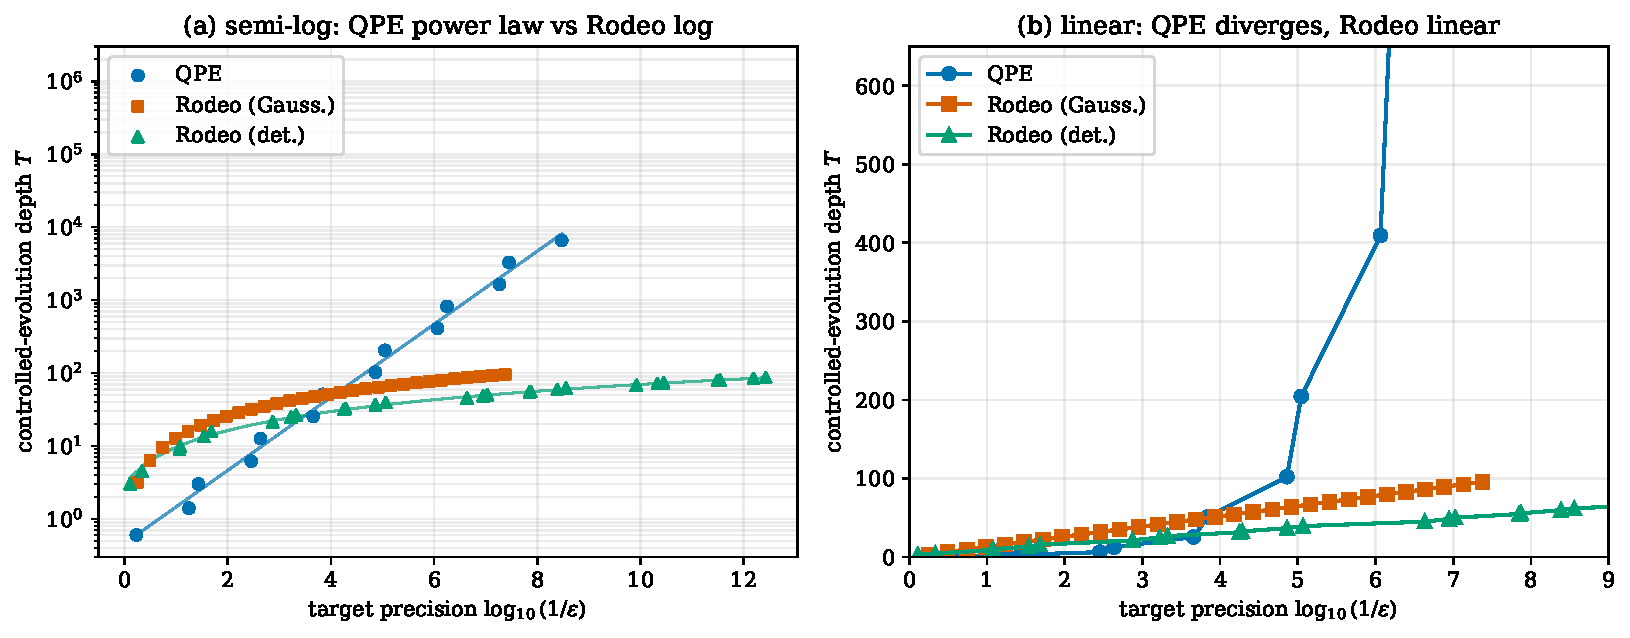
\includegraphics[width=\columnwidth]{fig_cost.pdf}
\caption{Resource cost of the zero-sector filter as a function of the target
precision $\log_{10}(1/\varepsilon)$ for the single-spin model ($h=0.5$, $g=1/2$).
Since the horizontal axis counts target digits, the approximately linear growth of
the Rodeo curves reflects the logarithmic dependence
$T_{\rm Rodeo}=O(\log(1/\varepsilon)/g)$, whereas the phase-estimation depth grows
rapidly according to its power-law dependence on $1/\varepsilon$. The deterministic
low-discrepancy schedule gives a single exact value for each filtering-step count;
for the Gaussian schedule we plot the analytic expected residual weight
$\mathbb{E}[|\beta_j|^2]$. Gate counts differ only by the common $(2N{+}1)^k$
prefactor.}
\label{fig:cost}\end{figure}

% ---- Figure 2 — fig_obs_error.pdf ----
\begin{figure}[tbp]\centering
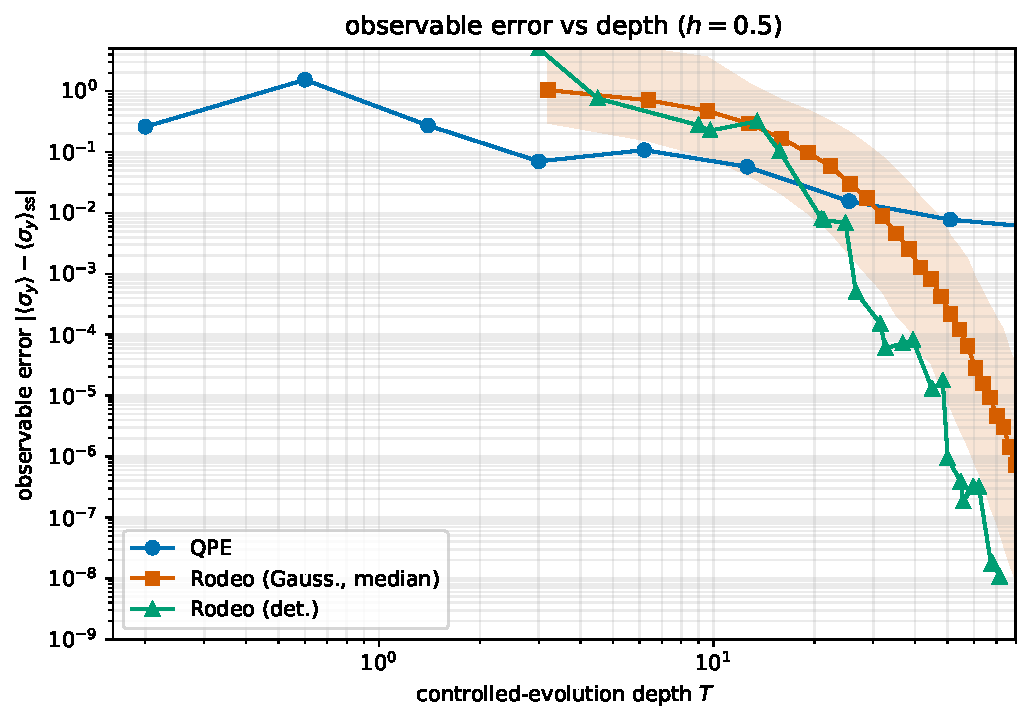
\includegraphics[width=\columnwidth]{fig_obs_error.pdf}
\caption{Single-shot observable error of $\langle\hat\sigma_y\rangle$ versus
controlled-evolution depth at $h=0.5$ (log--log). The phase-estimation filter is
shown as a line; for the Gaussian schedule we plot the median single-shot error with
its 10--90\% spread over random schedules. The deterministic schedule is exact. Both
Rodeo schedules cross below the phase-estimation curve at moderate depth and continue
to fall, while phase estimation plateaus, reflecting the logarithmic versus power-law
filtering cost.}
\label{fig:obs_error}\end{figure}

% ---- Figure 3 — fig_cost_vs_g.pdf ----
\begin{figure}[tbp]\centering
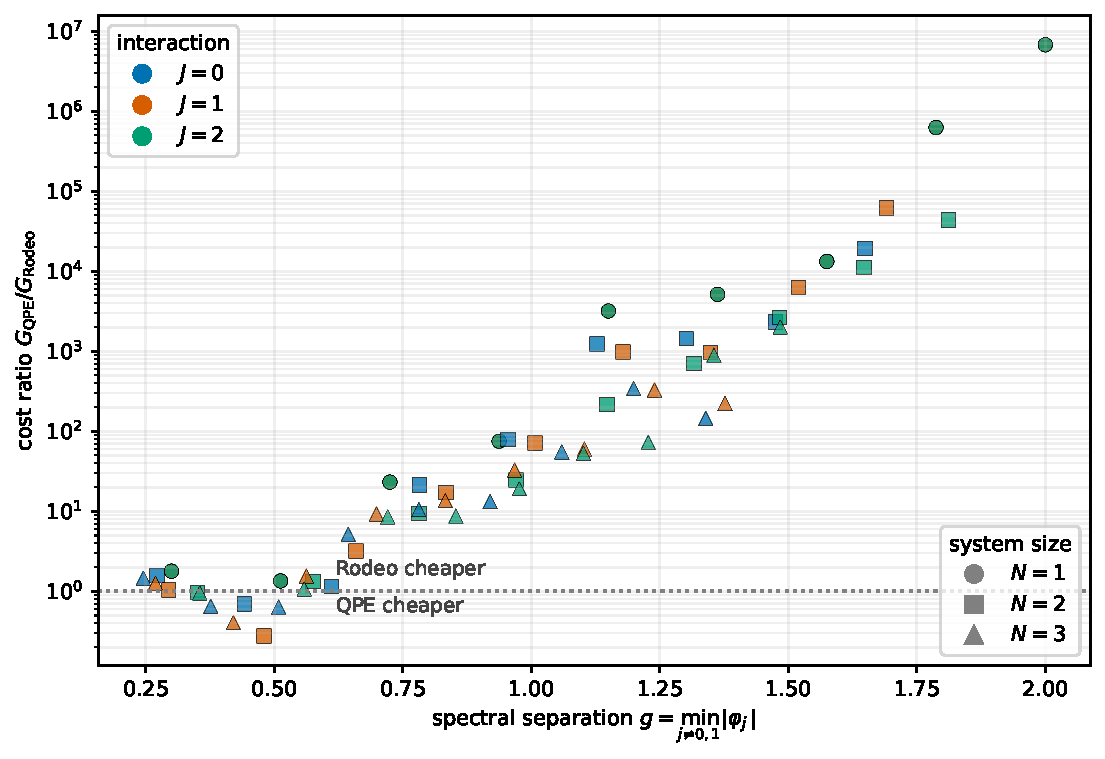
\includegraphics[width=\columnwidth]{fig_cost_vs_g.pdf}
\caption{Gate-cost ratio $G_{\rm QPE}/G_{\rm Rodeo}$ at fixed controlled-evolution
depth, as a function of the spectral separation $g$ of the embedding $M$. Each point
is a dissipative transverse-field Ising chain, swept over dissipation strength,
interaction strength $J$ (colour), and system size $N$ (marker). The data collapse
onto a single trend in $g$, and the Rodeo advantage grows with $g$. The dotted line
marks equal cost. The single-spin benchmark corresponds to $g=1/2$.}
\label{fig:cost_vs_g}\end{figure}

% ---- Figure 4 — fig_observables.pdf   (Appendix B) ----
\begin{figure*}[tbp]\centering
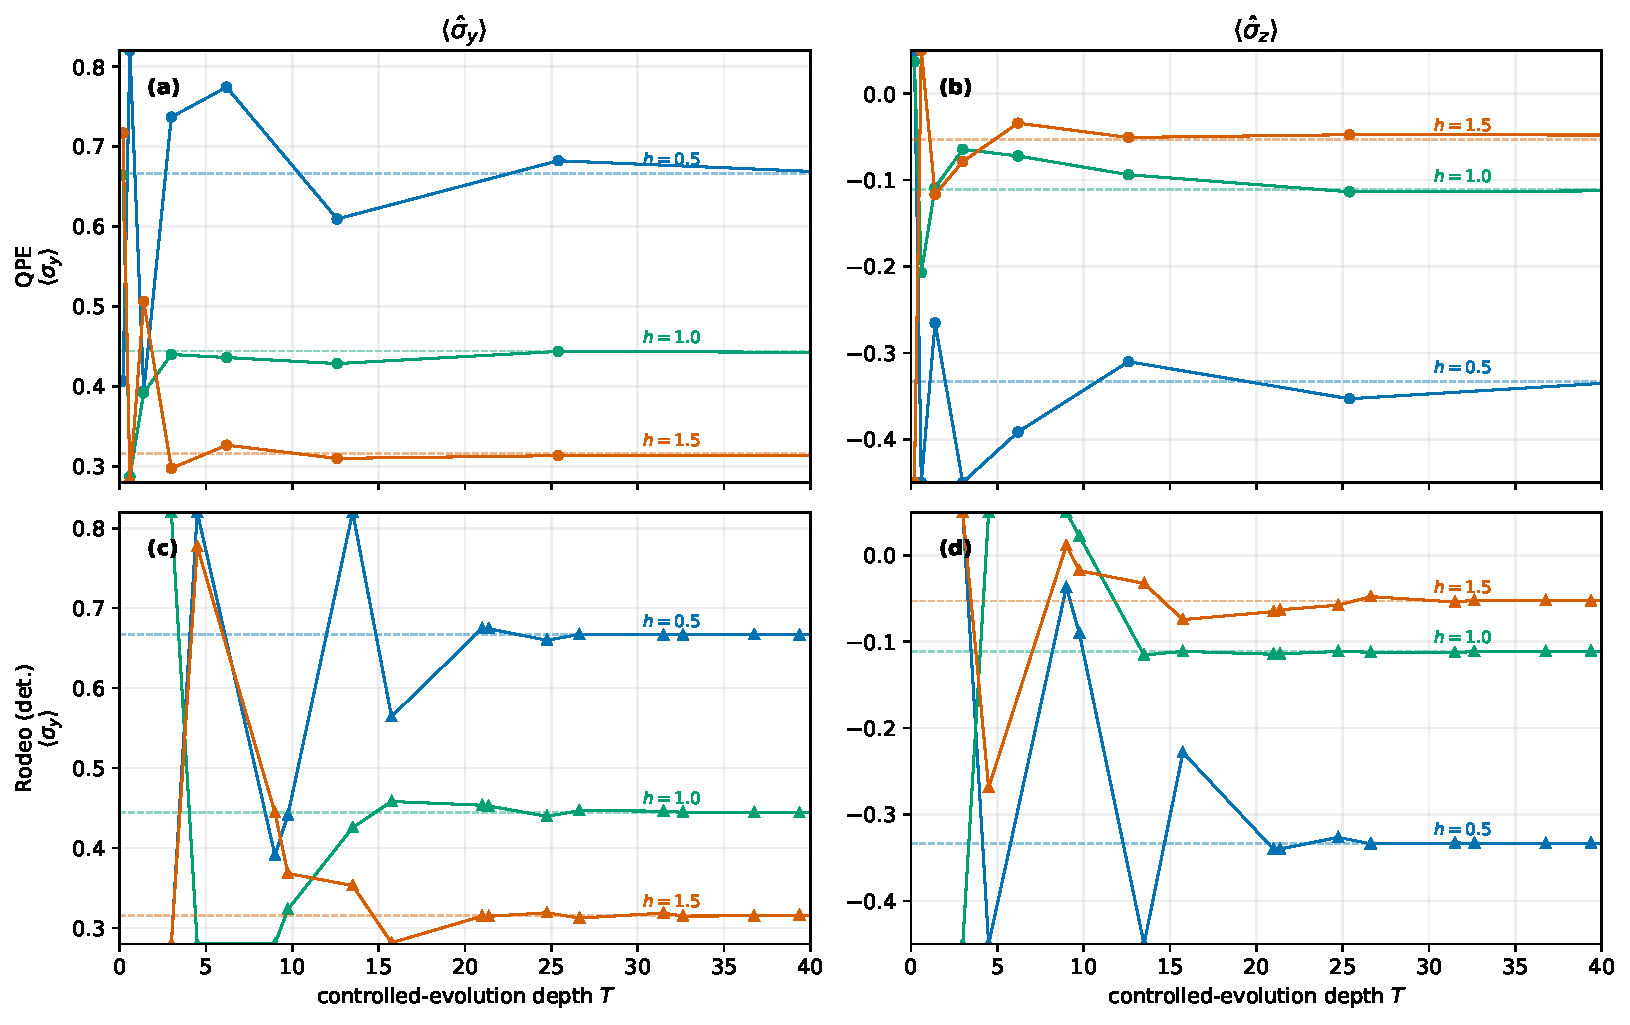
\includegraphics[width=\textwidth]{fig_observables.pdf}
\caption{Steady-state observables across the field values $h\in\{0.5,1.0,1.5\}$,
with each $h$ drawn in a distinct colour. Top row [(a),(b)]: phase estimation
(circles); bottom row [(c),(d)]: deterministic Rodeo filtering (triangles). Left
column [(a),(c)]: $\langle\hat\sigma_y\rangle$; right column [(b),(d)]:
$\langle\hat\sigma_z\rangle$. These are the two physically independent non-trivial
observables of the model, since $\langle\hat\sigma_x\rangle=0$ identically. The
estimates obtained from the ratio readout converge to the distinct exact NESS values
(dashed lines) as the controlled-evolution depth $T$ increases. The vertical axes are
restricted to the convergence window; at small depth the ratio estimator swings
strongly because the normalization readout passes near zero. Both filters reach the
same exact steady state, while the resource advantage of Rodeo filtering is quantified
in Fig.~\ref{fig:cost}.}
\label{fig:observables}\end{figure*}

% ---- Figure 5 — fig_collapse_decay_vs_g.pdf   (Appendix C.1) ----
% CORRECTED caption: panel (b) is the variance-explained bar (see discrepancy 1).
\begin{figure}[tbp]\centering

\includegraphics[width=\columnwidth]{fig_collapse_decay_vs_g.pdf}
\caption{Cost ratio $G_{\rm QPE}/G_{\rm Rodeo}$ at fixed controlled-evolution depth
over a $(\gamma,N,J)$ grid. \emph{(a)} When plotted against the Liouvillian decay rate
$g_{\rm decay}=\min|\re\,\lambda|$, the data scatter and separate systematically with
system size. \emph{(b)} Fraction of the variance of
$\log_{10}(G_{\rm QPE}/G_{\rm Rodeo})$ explained by each control variable alone
(single-variable $R^2$): the spectral separation $g$ explains $0.95$, far more than
the dissipation $\gamma$ ($0.73$), the decay rate $g_{\rm decay}$ ($0.65$), the system
size $N$ ($0.17$), or the interaction $J$ ($<0.01$). This identifies $g$, rather than
the asymptotic decay rate or any microscopic parameter, as the relevant resolution
scale for the filter-cost comparison.}
\label{fig:collapse}\end{figure}

% ---- Figure 6 — fig_interacting_collapse.pdf   (Appendix C.2) ----
% CORRECTED caption: 2x2 grid over J, four fixed g per panel (see discrepancy 2).
\begin{figure}[tbp]\centering
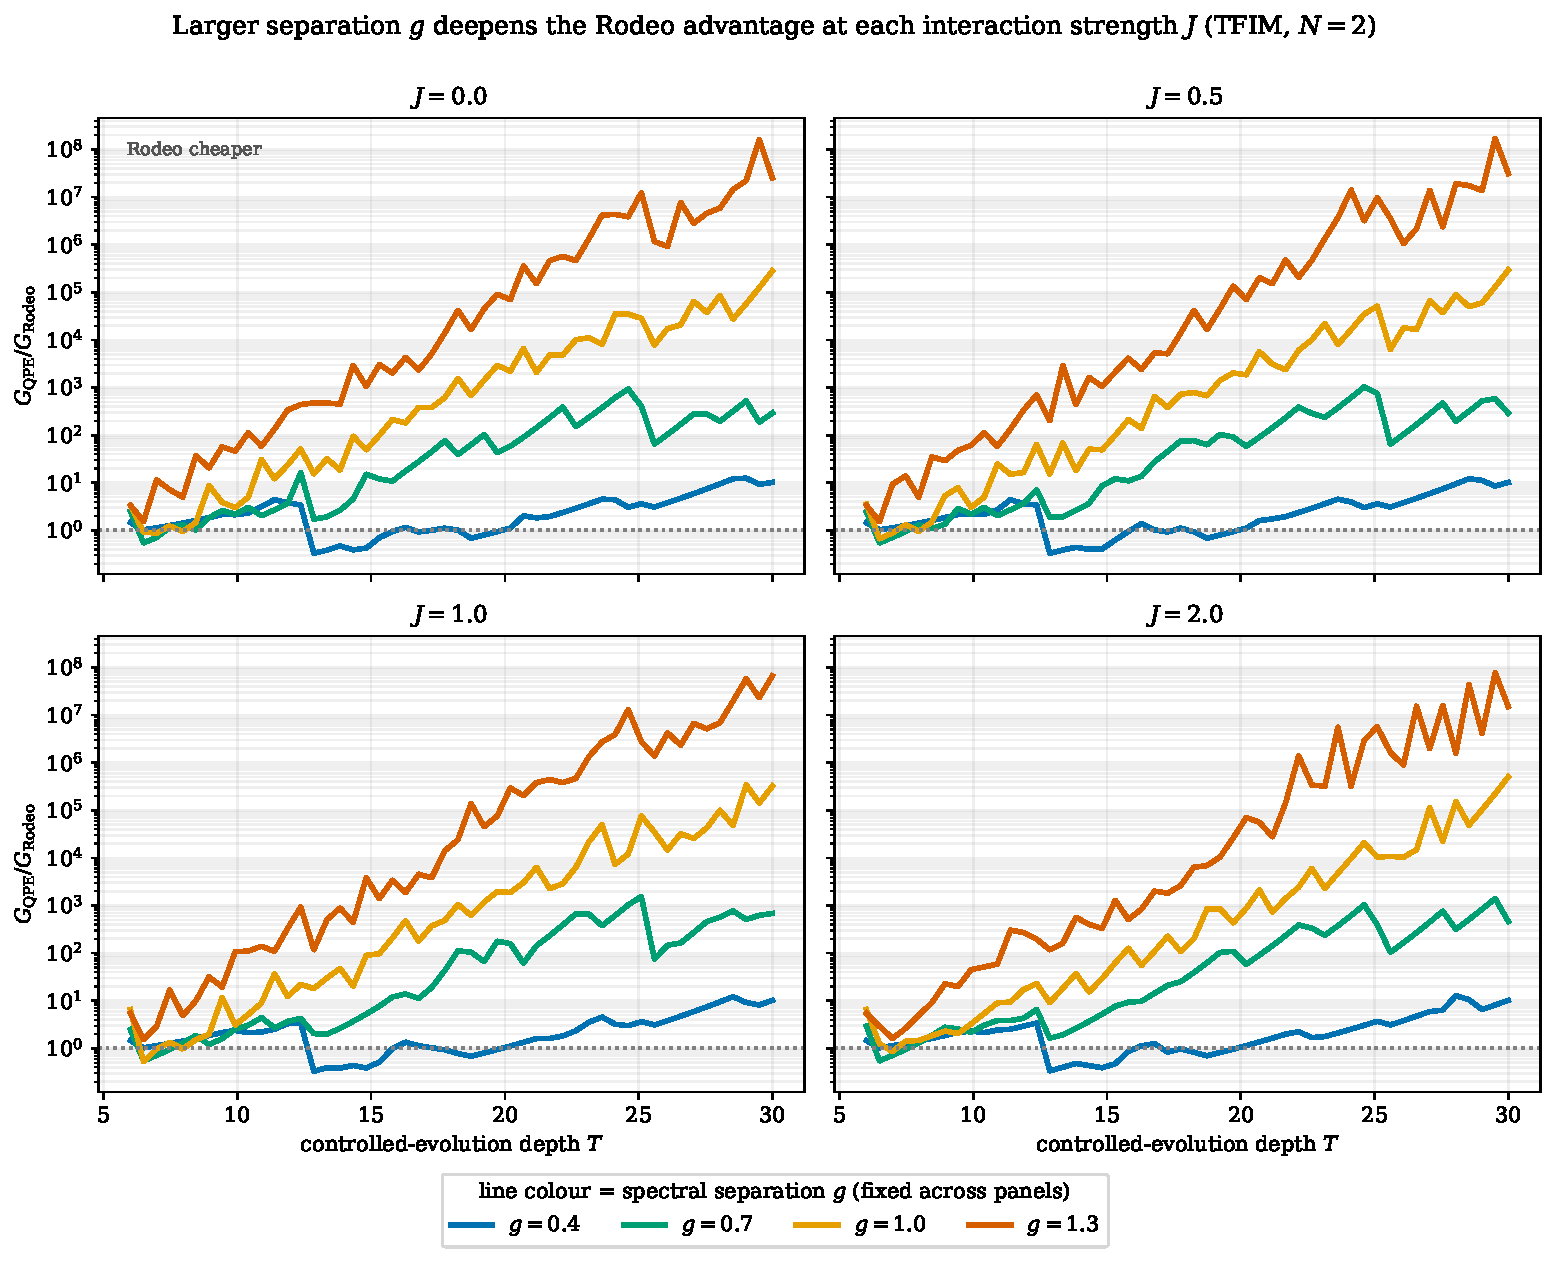
\includegraphics[width=\columnwidth]{fig_interacting_collapse.pdf}
\caption{The Rodeo advantage is organized by the spectral separation $g$ at every
interaction strength (dissipative transverse-field Ising model, $N=2$). Each panel
fixes the interaction $J$; within a panel the cost ratio $G_{\rm QPE}/G_{\rm Rodeo}$
is plotted versus controlled-evolution depth $T$ for four fixed separations $g$ (one
colour each, the same four values in every panel). The same-colour curve barely moves
from panel to panel: at fixed $g$ the advantage and its growth with $T$ are
essentially the same from $J=0$ to $J=2$, so the interaction is not an independent
control once $g$ is fixed.}
\label{fig:interacting}\end{figure}

% ---- Figure 7 — fig_density_saturation.pdf   (Appendix C.3) ----
\begin{figure}[tbp]\centering

\includegraphics[width=\columnwidth]{fig_density_saturation.pdf}
\caption{Spectral-density dependence at fixed embedding separation, using synthetic
spectra. Increasing the number of embedding modes changes the cost ratio most strongly
for the first few modes and then saturates. The separation $g$ sets the overall scale
of the Rodeo advantage, while the spectral density contributes a finite-spectrum
correction.}
\label{fig:density}\end{figure}


% =====================  SUPPLEMENT  ==================================

% ---- Figure S1 — rodeo_dynamic_circuit.pdf ----
\begin{figure}[tbp]\centering
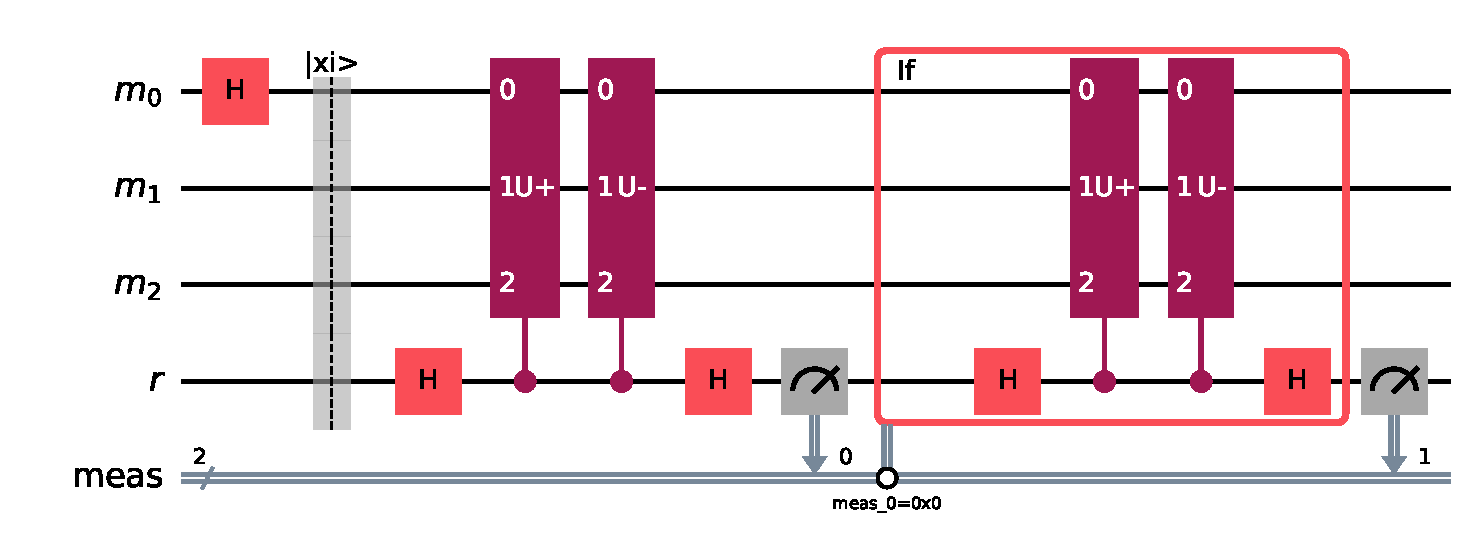
\includegraphics[width=\columnwidth]{rodeo_dynamic_circuit.pdf}
\caption{Dynamic Rodeo filter circuit for the single-spin embedding $M$, shown for two
cycles ($n=2$) and drawn from the compiled Qiskit circuit. The data register is
$\mathsf{m}=(\mathrm{row},\mathrm{col},\mathrm{branch})$, the Rodeo ancilla is reused
as $\mathsf{r}$, and the success bits are stored in the classical register
$\mathsf{meas}$. The controlled-evolution gates are $U_\pm\equiv e^{\pm iM t_\ell/2}$.
Each cycle applies $H$ on the ancilla, the symmetric evolutions $U_\pm$, a second $H$,
and a mid-circuit measurement. Later cycles sit inside a classically controlled block,
so a failed cycle aborts the remaining controlled evolutions. Each success-bit
measurement is placed outside the conditional, as required by current dynamic-circuit
restrictions, and failed shots are removed by post-selection.}
\label{fig:s_circuit}\end{figure}

% ---- Figure S2 — rodeo_trotter_decomp.pdf ----
\begin{figure}[tbp]\centering
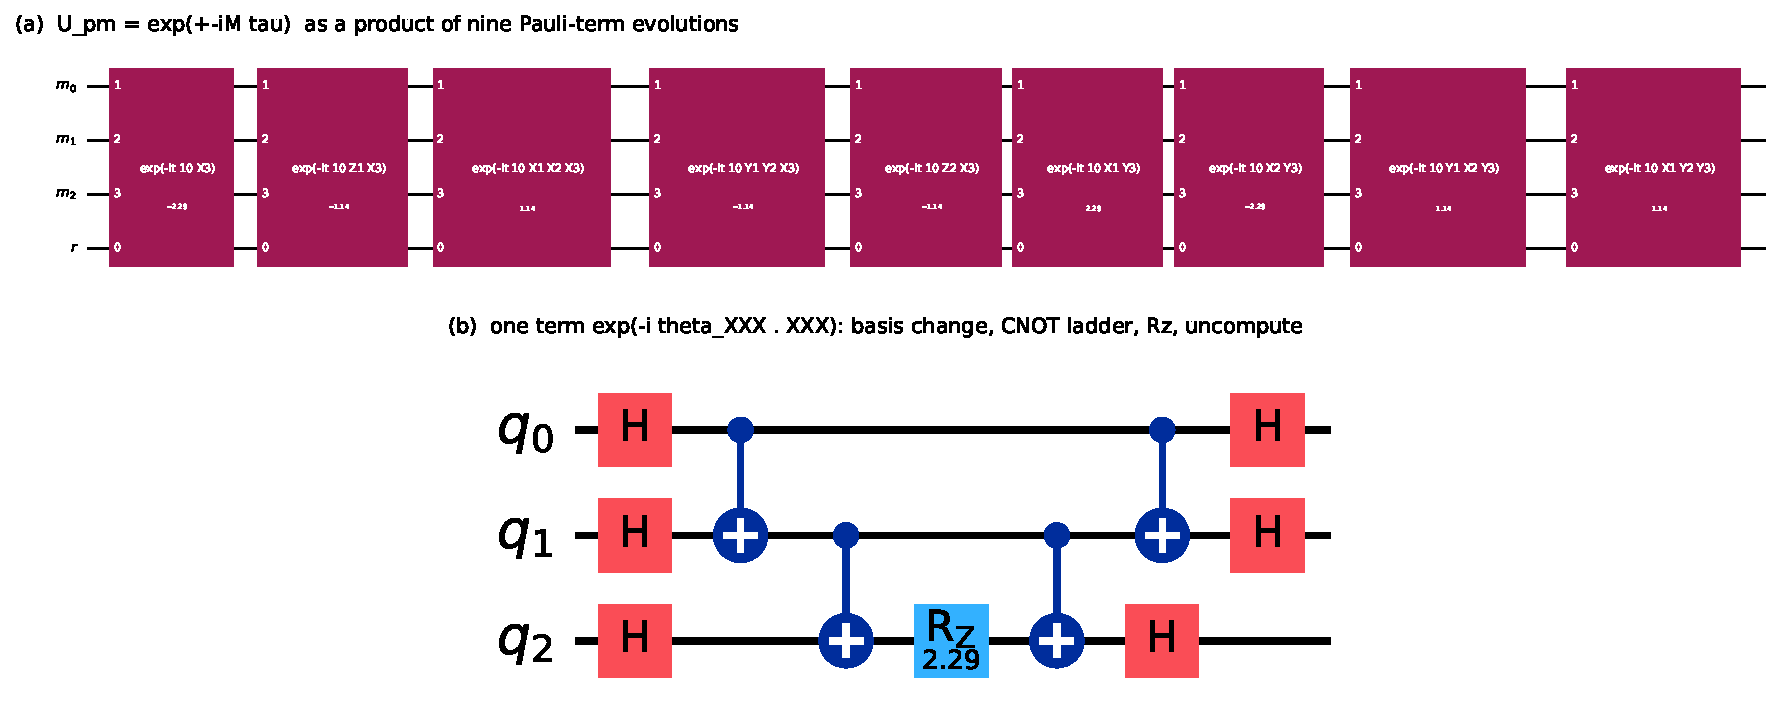
\includegraphics[width=\columnwidth]{rodeo_trotter_decomp.pdf}
\caption{Trotter realization of one Rodeo controlled evolution for the single-spin
embedding $M$, drawn from the compiled Qiskit circuit. The controlled evolution
$U_\pm=e^{\pm iM\tau}$ is written as a product of Pauli-term evolutions
$e^{-i\theta_P P}$ with
$P\in\{XII,\,XIZ,\,XXX,\,XYY,\,XZI,\,YIX,\,YXI,\,YXY,\,YYX\}$. Each term expands into
basis changes, a CNOT ladder, an $R_z$ phase rotation, and the uncomputing ladder.}
\label{fig:s_trotter}\end{figure}

% ---- Figure S3 — aer_convergence.pdf ----
\begin{figure}[tbp]\centering
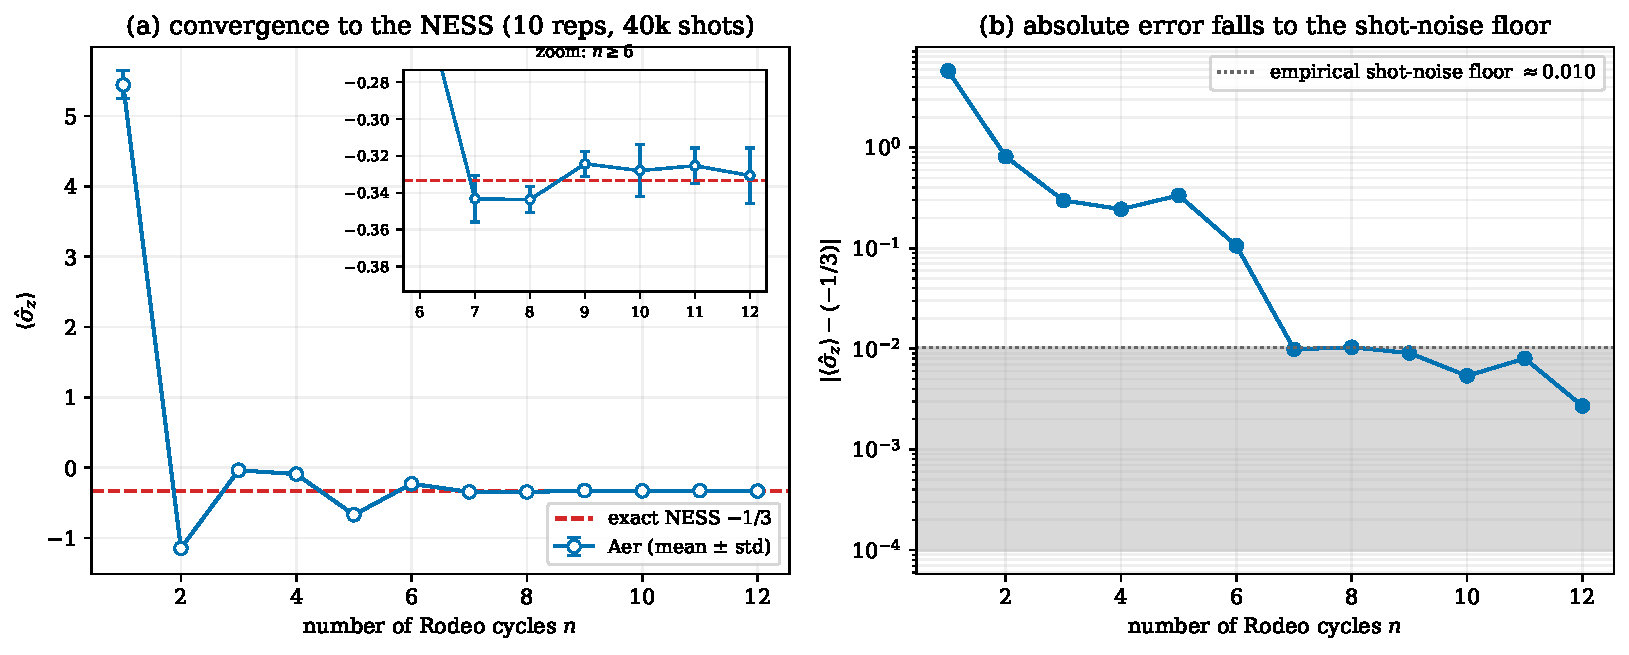
\includegraphics[width=\columnwidth]{aer_convergence.pdf}
\caption{Statevector circuit check on the single-spin model ($h=0.5$, $g=1/2$).
\emph{(a)} The post-selected ratio estimate of $\langle\hat\sigma_z\rangle$ from the
compiled dynamic Rodeo circuit converges to the exact NESS value $-1/3$ as the number
of cycles $n$ increases; markers are the mean over independent noiseless runs and the
error bars are the empirical run-to-run standard deviation (inset: zoom for $n\geq6$).
The transient oscillation at small $n$ reflects incomplete, sign-alternating
suppression of nonzero modes by the finite schedule. \emph{(b)} The absolute error on
a logarithmic scale falls to the empirical shot-noise floor, approximately $10^{-2}$
for $4\times10^{4}$ shots, once the spectral separation is resolved.}
\label{fig:s_convergence}\end{figure}

% ---- Figure S4 — aer_cycle_saving.pdf ----
% CORRECTED caption: saving rises toward 3/7 ~ 43%, not "saturates near 25%"
% (see discrepancy 3).
\begin{figure}[tbp]\centering
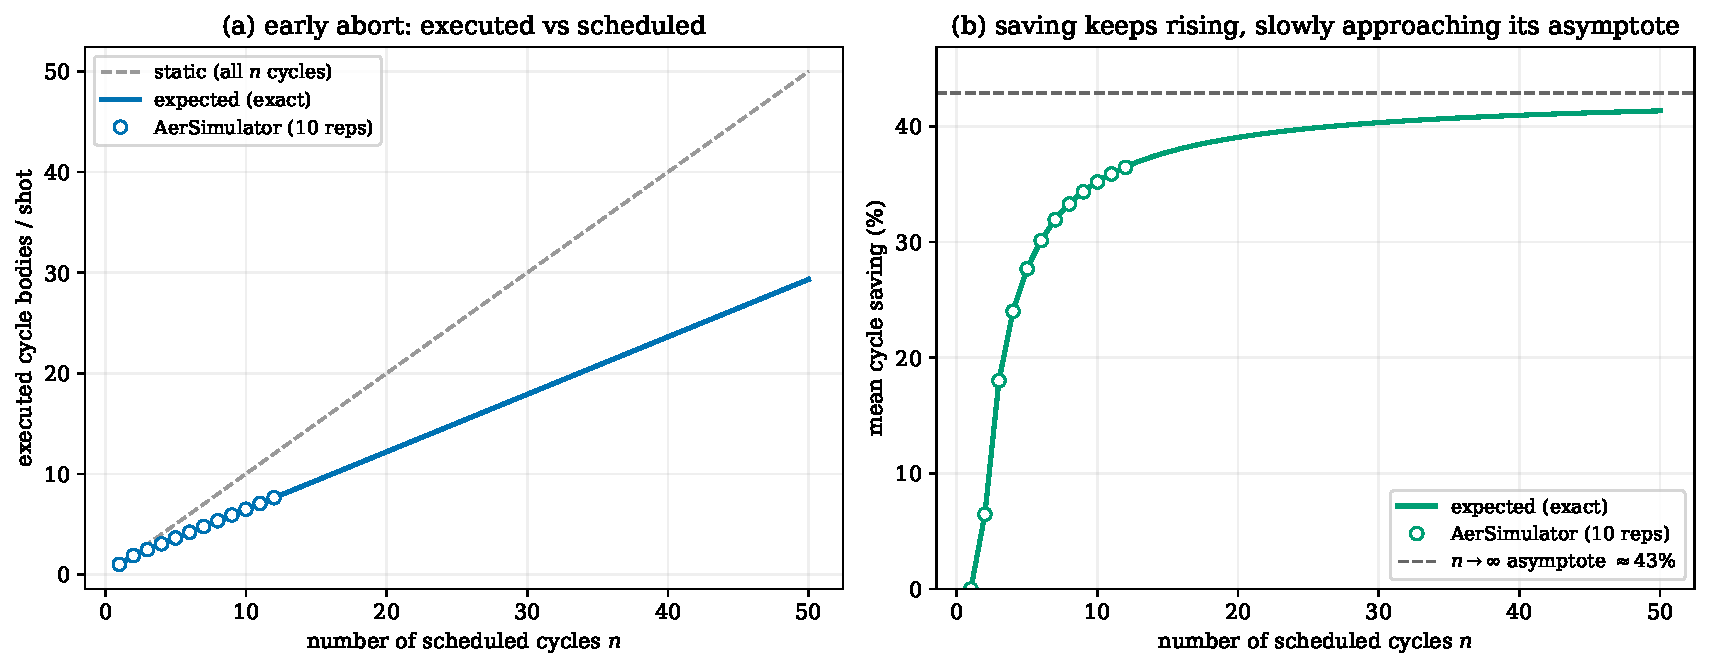
\includegraphics[width=\columnwidth]{aer_cycle_saving.pdf}
\caption{Gate-level early-abort saving for the dynamic Rodeo circuit ($h=0.5$). The
solid curve is the exact expected value computed on the statevector (no sampling); the
open markers are the noiseless \texttt{AerSimulator} means, which validate it.
\emph{(a)} Mean number of Rodeo cycle bodies executed per shot (dynamic, with early
abort) versus the static cost of running all $n$ cycles. \emph{(b)} The resulting mean
cycle saving rises monotonically with the scheduled depth and slowly approaches a
finite asymptote ($3/7\approx43\%$, dashed); it does \emph{not} saturate near $25\%$,
and the early-abort benefit keeps growing well beyond the depths reached by the circuit
simulation. The effect follows from the measurement-conditioned circuit structure and
is the circuit-level counterpart of the restart-on-failure advantage analysed in the
main text.}
\label{fig:s_saving}\end{figure}
